\label{sec:results}
In this section we briefly present the results obtained.
The agent communicates correctly with the virtual robot and manages to complete its task completely.
It is possible to see the operation of the framework in two videos, \href{https://youtu.be/dQbiNx36fNs}{one} in which the agent simply performs its task and \href{https://youtu.be/iuQfDgS0oUE}{one} in which the debug mode is activated in which we can see the paths calculated by the robot.

\begin{figure}
    \centering
    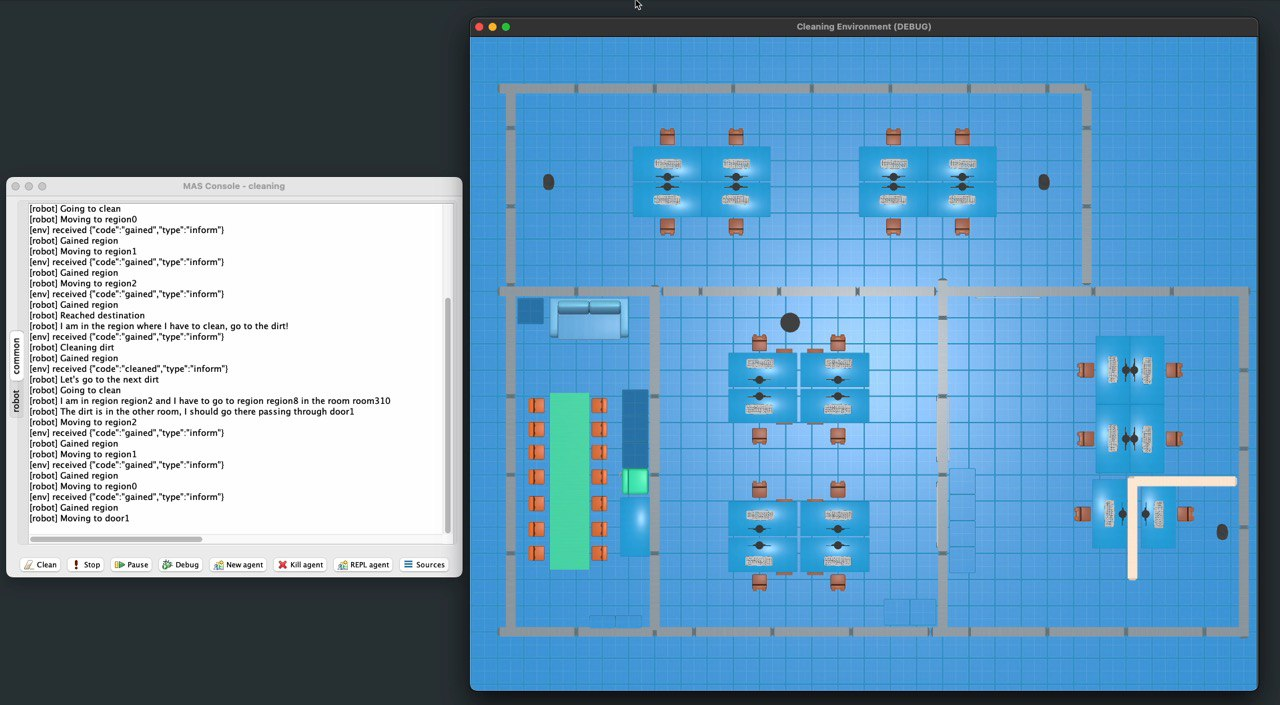
\includegraphics[width=\textwidth]{sections/imgs/screen.jpeg}
    \caption{The agent in action.}
    \label{fig:screen}
\end{figure}
In the Figure\ref{fig:screen} you can see the framework in action.
On the left is the JaCaMo window in which the agent is implemented while on the right is visible Godot and the robot you want in the room.

In the implementation we were able to completely separate the logical reasoning part from the coordinate management part.
For the time being, however, the agent is still not looking for the best path but simply for a walkable path from one region to another.
The results confirm that the robot in this way has full freedom of rotation by producing non-regular paths and that the ability to find paths in the instrument continuum is enhanced.
The robot's path planning, in addition to the features already listed, also has the ability to adapt to any occlusions dynamically, recalculating the path in case something has moved without having to take it into account logically.

This implementation is easily scalable from both the environment and multi-agent system perspectives.
In fact, the region-based logic model makes it very easy to expand the environment both in width and depth (increasing its accuracy); in fact, we have already demonstrated the operation of subregions by implementing rooms.
The connection between agent and robot implemented end-to-end with a private artifact of the agent and a proven script of the robot also makes the multi-agent system scalable without the need for further major modifications.